\label{chap:background}

There are different types optimizations that can be performed on a program to improve its
performance. The optimization can be made for finding data locality and hence extracting
parallelism. Starting from the early history of programming languages the internal representation
of program is done with Abstract Syntax Tree(AST). Though some elementary transformation can
be performed on AST it is tough to carry out complex transformations like dependency analysis among
statements inside a loop. Trees are very rigid data structures to do such transformations.
In this chapter a extremely powerful mathematical model which puts together analysis power,expressiveness and flexibility is explained in detail.

\section{Program Transformations with polyhedral model}

In this section some of the common program transformations which can be realized with the
assistance of polyhedral model are explained. The polyhedral model is not a normal representation of programs when compared to the
classical structure of programs(like AST) that every programmer is familiar with. But
it is easier to do transformations smoothly in this model.

\subsection{Transformation for improving data locality}

The polyhedral model can detect common array accesses which improves the data locality. It is
illustrated with a simple example.
{\footnotesize
\begin{lstlisting}
  for(i = 1; i <= 10; i++)
    A[i] = 10;
  
  for(j = 6; j <= 15; j++)
    A[j] = 15;
\end{lstlisting}
}

The two loops will be represented by two polyhedrons and it can find the common 
array accesses starting from index 6 to 10 and the code can be transformed as follows.

{\footnotesize
\begin{lstlisting}

for(i = 1; i <= 5; i++)
  A[i] = 10;

for(j = 6; j <= 15; j++)
  A[j] = 15;
\end{lstlisting}
}

\subsection{Scalar Expansion}

----Give example gsoc----

\subsection{Constant propagation through arrays}
\subsection{Eliminate dead loop iterations}
\subsection{Automatic parallelization}
\subsection{Vectorization}

\section{Polyhedral representation of Programs}

The polyhedral model does its transformations based on linear algebra and linear programming.
Certain parts of programs known as SCoPs(Static control Part) are represented in this model.
A program part that can be represented using polyhedral model is called SCoPs. Generally
loops are the candidates for SCoPs. There are some restrictions to the set of statements 
in the section of code to be qualified as SCoP. Those are listed below.

\begin{itemize}
\item The set of statements in the loops should have bounds and conditionals having affine functions
of surrounding iterators and the parameters (constants whose values are unknown at compile time).
\item There should be structured control flow.
\item Side effect free(Only pure functions are allowed)
\end{itemize}

There are efforts to increase the application domain of polyhedral model \cite{Benabderrahmane}
which shows most of the restrictions are artificial.

There are three parts to this representation.
\begin{figure}
  \label{fig:poly_steps}
  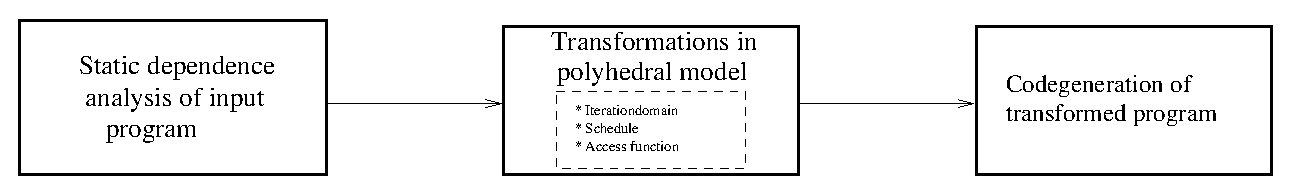
\includegraphics[width=1\textwidth]{images/poly_steps.eps}
  \caption{Transformation in polyhedral model}
\end{figure}

\subsection{Iteration Domain}
\subsection{The Schedule}
\subsection{Access function}
